\documentclass{beamer}\usepackage[]{graphicx}\usepackage[]{color}
%% maxwidth is the original width if it is less than linewidth
%% otherwise use linewidth (to make sure the graphics do not exceed the margin)
\makeatletter
\def\maxwidth{ %
  \ifdim\Gin@nat@width>\linewidth
    \linewidth
  \else
    \Gin@nat@width
  \fi
}
\makeatother

\definecolor{fgcolor}{rgb}{0.345, 0.345, 0.345}
\newcommand{\hlnum}[1]{\textcolor[rgb]{0.686,0.059,0.569}{#1}}%
\newcommand{\hlstr}[1]{\textcolor[rgb]{0.192,0.494,0.8}{#1}}%
\newcommand{\hlcom}[1]{\textcolor[rgb]{0.678,0.584,0.686}{\textit{#1}}}%
\newcommand{\hlopt}[1]{\textcolor[rgb]{0,0,0}{#1}}%
\newcommand{\hlstd}[1]{\textcolor[rgb]{0.345,0.345,0.345}{#1}}%
\newcommand{\hlkwa}[1]{\textcolor[rgb]{0.161,0.373,0.58}{\textbf{#1}}}%
\newcommand{\hlkwb}[1]{\textcolor[rgb]{0.69,0.353,0.396}{#1}}%
\newcommand{\hlkwc}[1]{\textcolor[rgb]{0.333,0.667,0.333}{#1}}%
\newcommand{\hlkwd}[1]{\textcolor[rgb]{0.737,0.353,0.396}{\textbf{#1}}}%
\let\hlipl\hlkwb

\usepackage{framed}
\makeatletter
\newenvironment{kframe}{%
 \def\at@end@of@kframe{}%
 \ifinner\ifhmode%
  \def\at@end@of@kframe{\end{minipage}}%
  \begin{minipage}{\columnwidth}%
 \fi\fi%
 \def\FrameCommand##1{\hskip\@totalleftmargin \hskip-\fboxsep
 \colorbox{shadecolor}{##1}\hskip-\fboxsep
     % There is no \\@totalrightmargin, so:
     \hskip-\linewidth \hskip-\@totalleftmargin \hskip\columnwidth}%
 \MakeFramed {\advance\hsize-\width
   \@totalleftmargin\z@ \linewidth\hsize
   \@setminipage}}%
 {\par\unskip\endMakeFramed%
 \at@end@of@kframe}
\makeatother

\definecolor{shadecolor}{rgb}{.97, .97, .97}
\definecolor{messagecolor}{rgb}{0, 0, 0}
\definecolor{warningcolor}{rgb}{1, 0, 1}
\definecolor{errorcolor}{rgb}{1, 0, 0}
\newenvironment{knitrout}{}{} % an empty environment to be redefined in TeX

\usepackage{alltt}
%\usepackage{alltt}
\usepackage[utf8]{inputenc}
\usepackage[brazilian]{babel}
\usepackage{amsmath}
\usepackage{amssymb} % para símbolos
\usepackage{enumerate}
\usepackage{cancel}%para usar o cancelamento
\usetheme{Madrid}

\renewcommand{\CancelColor}{\color{red}}
\IfFileExists{upquote.sty}{\usepackage{upquote}}{}
\begin{document}
	\title{Lista 2}
	\subtitle{Tópicos Especiais em Engenharia de Computação}
	\author{Eric Calasans de Barros \and  Fagner Ferreira}
	
	\begin{frame}[plain]
		\maketitle
	\end{frame}
	
	\section{Questão 1}
		\begin{frame}
			\frametitle{Questão 1}
			Sejam $\bar{x}_{1} = 230,0 s_{1} = 10,7, \bar{x}_{2} = 225,5, s_{1} = 10,7 e s_{2} = 15,4$, para $\sigma_{1}^{2} = \sigma_{2}^{2}$, calcularemos um \textbf{intervalo de confiança(IC)} de 95\%($\alpha = 0.05$) para a diferença das médias $\mu_{1} - \mu_{2}$.  Se $$s = \frac{\sigma}{\sqrt{n}}$$
			
			então:
			
			$$Z = \frac{\bar{x} - \mu}{\sigma/\sqrt{n}} = \frac{\bar{x} - \mu}{s} \Rightarrow \mu = \bar{x} \pm Z*s$$
		\end{frame}
		\begin{frame}
			\frametitle{Questão 1}
			Dizer que a média está contida num determinado IC significa que $\mu = \bar{x} \pm Zs$.  Assim, para a diferença das médias temos que:
				\begin{align*}
					\mu_{1} - \mu_{2} &= (\bar{x}_{1} \pm Zs_{1}) - (\bar{x}_{2} \pm Zs_{2})\\
					&= \bar{x}_{1} \pm  Zs_{1} - \bar{x}_{2} \pm Zs_{2}\\
					&= (\bar{x}_{1} - \bar{x}_{2}) \pm Z(s_{1} - s_{2})
				\end{align*}
				
				Como procuramos um IC bilateral temos que $\frac{\alpha}{2} = 0.025$.  Pela simetria da curva de distribuição Normal temos que $|Z_{\alpha}| = |Z_{1-\alpha}| \Rightarrow |Z_{0,025}| = |Z_{0,975}|$.  
                \end{frame}
                
                \begin{frame}[fragile]
                        \frametitle{Questão 1}
                        Com a ajuda do software estatístico RStudio:
\begin{knitrout}
\definecolor{shadecolor}{rgb}{0.969, 0.969, 0.969}\color{fgcolor}\begin{kframe}
\begin{alltt}
\hlkwd{qnorm}\hlstd{(}\hlnum{.975}\hlstd{)}
\end{alltt}
\begin{verbatim}
## [1] 1.959964
\end{verbatim}
\end{kframe}
\end{knitrout}
                        Assim temos:
                        $$\mu_{1} - \mu_{2} = (230,0 - 225,5)\pm1,96(10,7-15,4) = 7,5\pm9,2$$

                \end{frame}
                
    \section{Questão 2}
    	\begin{frame}
    		\frametitle{Questão 2}
    		Sejam $n_{1} = 20, \bar{x}_{1} = 510, s^{2}_{1} = 20$ e $n_{2} = 15, \bar{x}_{2} = 620, s^{2}_{2} = 30$ com $\sigma_{1}^{2} \neq \sigma_{2}^{2}$., deseja-se calcular:\\
    		\begin{enumerate}[a)]
    			\item \textbf{{Um intervalo de confiança de 95\% para}} $\boldsymbol{\mu_{1} - \mu_{2}}$\\
    			
    			Como $n \leq 30$ em ambos os casos, usamos uma distribuição \textbf{t-Student}.  Assim, para $\sigma_{1}^{2} \neq \sigma_{2}^{2}$ temos que $$\mu_{1}-\mu_{2} = (\bar{x}_{1} - \bar{x}_{2}) \pm t_{df}\sqrt{\frac{s_{1}^{2}}{n_{1}}+\frac{s_{2}^{2}}{n_{2}}}$$
    			
    			onde $$d_{f} = \frac{(\frac{s_{1}^{2}}{n_{1}}+\frac{s_{2}^{2}}{n_{2}})}{\frac{(\frac{s_{1}^{2}}{n_{1}})^2}{n_{1}-1} + \frac{(\frac{s_{2}^{2}}{n_{2}})^2}{n_{2}-1}} = \frac{(20/20 + 30/15)^2}{\frac{(20/20)^2}{19}+\frac{(30/15)^2}{14}} = 26$$ 
    			
    		\end{enumerate}
    	\end{frame}
    	
    	\begin{frame}[fragile]
    		\frametitle{Questão 2}
    		\begin{enumerate}[a)]
    			\item cont.$$\mu_{1} - \mu_{2} = (\bar{x}_1) - \bar{x}_2)\pm t_{0,975,26}\sqrt{\frac{s_{1}^{2}}{n_{1}}+\frac{s_{2}^{2}}{n_{2}}}$$
    			
    			Pelo \textbf{RStudio}:
\begin{knitrout}
\definecolor{shadecolor}{rgb}{0.969, 0.969, 0.969}\color{fgcolor}\begin{kframe}
\begin{alltt}
\hlkwd{qt}\hlstd{(}\hlnum{.975}\hlstd{,}\hlnum{26}\hlstd{)}
\end{alltt}
\begin{verbatim}
## [1] 2.055529
\end{verbatim}
\end{kframe}
\end{knitrout}
    		\begin{align*}
		        \mu_{1} - \mu_{2} &= (510 - 620) \pm 2,056\sqrt{\frac{20}{20} + \frac{30}{15}}\\
			&= -110 \pm 3,561
				\end{align*}
    		\end{enumerate}
    	\end{frame}
    	
    	\begin{frame}
    		\frametitle{Questão 2}
    		\begin{enumerate}[b)]
    			\item Dadas $\sigma_{1}^{2}$ e $\sigma_{2}^{2}$ as variânicas de duas V.A.s com distribuição normal e $s_{1}^2$ e $s_{2}^{2}$ as variâncias amostrais, define-se \textbf{F} com \textbf{distribuição F de Snedecom}:
    		$$\boldsymbol{F = \frac{s^{2}_{1}/\sigma_{1}^{2}}{s^{2}_{2}/\sigma_{2}^{2}} = \frac{s^{2}_{1}}{s^{2}_{2}} \frac{\sigma_{2}^{2}}{\sigma_{1}^{2}}}$$ 
    			para os graus de liberdade $df_{1} = m-1$ e $df_{2} = n-1$\\
    			Para construir um IC a variável F deve obedecer à seguinte probabilidade:
    			$$\boldsymbol{P(F_{\frac{\alpha}{2},df_{1},df_{2}} < F < F_{1-\frac{\alpha}{2},df_{1},df_{2}}) = 1 - \alpha}$$
    		\end{enumerate}	
    	\end{frame}
    
    	\begin{frame}
	    	\frametitle{Questão 2}
	    	\begin{enumerate}[b)]
	    		\item \textit{cont.}\\
	    			Para tanto:
	    			\begin{align*}
		    			F_{\frac{\alpha}{2},df_{1},df_{2}} < &\frac{s^{2}_{1}}{s^{2}_{2}} \frac{\sigma_{2}^{2}}{\sigma_{1}^{2}} < F_{1-\frac{\alpha}{2},df_{1},df_{2}}\\   
		    			F_{\frac{\alpha}{2},df_{1},df_{2}} \frac{s^{2}_{2}}{s^{2}_{1}}< & \frac{\sigma_{2}^{2}}{\sigma_{1}^{2}} < F_{1-\frac{\alpha}{2},df_{1},df_{2}}\frac{s^{2}_{2}}{s^{2}_{1}}
	    			\end{align*}
	    			Invertendo os termos:$$\boldsymbol{\frac{1}{F_{1-\frac{\alpha}{2},df_{1},df_{2}}}\frac{s^{2}_{2}}{s^{2}_{1}} < \frac{\sigma_{1}^{2}}{\sigma_{2}^{2}} < \frac{1}{F_{\frac{\alpha}{2},df_{1},df_{2}}}\frac{s^{2}_{2}}{s^{2}_{1}}}$$
	    	\end{enumerate}	
    \end{frame}
	
	\begin{frame}[fragile]
		\frametitle{Questão 2}
		\begin{enumerate}[b)]
			\item \textit{cont.}\\
			Substituindo os valores:\\
			$$\frac{1}{F_{0.975,19,14}}\frac{20}{30} < \frac{\sigma_{1}^{2}}{\sigma_{2}^{2}} < \frac{1}{F_{0.975,19,14}}\frac{20}{30}$$
			Utilizando o \textbf{RStudio} e a propriedade da distribuição F:$$F_{\frac{\alpha}{2},df_{1},df_{2}} = \frac{1}{F_{1-\frac{\alpha}{2},df_{1},df_{2}}}$$
\begin{knitrout}
\definecolor{shadecolor}{rgb}{0.969, 0.969, 0.969}\color{fgcolor}\begin{kframe}
\begin{alltt}
\hlkwd{round}\hlstd{(}\hlkwd{qf}\hlstd{(}\hlnum{0.025}\hlstd{,}\hlnum{19}\hlstd{,}\hlnum{14}\hlstd{),}\hlkwc{digits} \hlstd{=} \hlnum{3}\hlstd{)}
\end{alltt}
\begin{verbatim}
## [1] 0.378
\end{verbatim}
\end{kframe}
\end{knitrout}
			
		\end{enumerate}
	\end{frame}
	
	\begin{frame}
		\frametitle{Questão 2}
		\begin{enumerate}[b)]
			\item \textit{cont.}\\
			$$F_{0.975,19,14} = \frac{1}{F_{0.025,19,14}} = \frac{1}{0.378} = 2.645$$
			
			Logo:
			\begin{align*}
				\frac{1}{2.645}\frac{20}{30} < &\frac{\sigma_{1}^{2}}{\sigma_{2}^{2}} < \frac{1}{0.378}\frac{20}{30}\\ 0.251 < &\frac{\sigma_{1}^{2}}{\sigma_{2}^{2}} < 1.754
			\end{align*}
		\end{enumerate}	
	\end{frame}
	
	\section{Questão 3}
	\begin{frame}
			\frametitle{Questão 3}
			Sejam $n = 300, \bar{x} = 1660$ e $s = 90h$, deseja-se testar:
			\begin{itemize}
				\item $\boldsymbol{H_{0}:  \mu_{0} = 1690h}$
				\item $\boldsymbol{H_{1}:  \mu_{0} \neq 1690h}$
			\end{itemize}
			Trata-se, portanto, de um \textbf{Teste Z bicaudal}.  Para:
			\begin{enumerate}[a)]
				\item $\alpha = 0.05$\\
				Calculadndo $Z = \frac{\bar{x} - \mu_{0}}{s/\sqrt{n}} = \frac{1660-1690}{90/\sqrt{300}} = -5,77$\\
				Conforme calculado em questão anterior:$$Z_{0.025} = -1.96 \hspace{0.5cm}Z_{0.975} = 1.96$$ 
				Como $ Z < Z_{\frac{\alpha}{2}}$ \textbf{rejeitamos H\textsubscript{0} com} $\boldsymbol{\alpha = 0.05}$  
			\end{enumerate}
		\end{frame}
		
		\begin{frame}[fragile]
			\frametitle{Questão 3}
			\begin{enumerate}[b)]
				\item $\alpha = 0.01$\\
				Para o mesmo $Z = -5.77$ e $Z_{\frac{\alpha}{2}} \ = Z_{\frac{0.01}{2}} = Z_{0.005} $
\begin{knitrout}
\definecolor{shadecolor}{rgb}{0.969, 0.969, 0.969}\color{fgcolor}\begin{kframe}
\begin{alltt}
\hlkwd{qnorm}\hlstd{(}\hlnum{0.025}\hlstd{)}
\end{alltt}
\begin{verbatim}
## [1] -1.959964
\end{verbatim}
\end{kframe}
\end{knitrout}
			Como $Z < Z_{\frac{\alpha}{2} }$ \textbf{rejeitamos H\textsubscript{0} com} $\boldsymbol{\alpha = 0.01}$
			\end{enumerate}
		\end{frame}
	\section{Questão 4}
	\begin{frame}[fragile]
			\frametitle{Questão 4}
			Sejam $n = 20, \bar{x} = 0.06$ e $s = 0.009$, deseja-se testar:
			\begin{itemize}
				\item $\boldsymbol{H_{0}:  \mu_{0} = 0.05pol}$
				\item $\boldsymbol{H_{1}:  \mu_{0} \neq 0.05pol}$
			\end{itemize}
			Trata-se, portanto, de um \textbf{Teste t bicaudal}.  Para:
			\begin{enumerate}[a)]
				\item $\alpha = 0.05$\\
				Calculadndo $t = \frac{\bar{x} - \mu_{0}}{s/\sqrt{n}} = \frac{0.06 - 0.05}{0.009/\sqrt{20}} = 4.969$\\
				Calculando $t_{1-\frac{\alpha}{2},19}$:
\begin{knitrout}
\definecolor{shadecolor}{rgb}{0.969, 0.969, 0.969}\color{fgcolor}\begin{kframe}
\begin{alltt}
\hlkwd{qt}\hlstd{(}\hlnum{0.975}\hlstd{,}\hlnum{19}\hlstd{)}
\end{alltt}
\begin{verbatim}
## [1] 2.093024
\end{verbatim}
\end{kframe}
\end{knitrout}
                        Como $t > t_{1-\frac{\alpha}{2}} $ \textbf{rejeitamos H\textsubscript{0} com} $\boldsymbol{\alpha = 0.05}$
			\end{enumerate}
		\end{frame}
		
		\begin{frame}[fragile]
			\frametitle{Questão 4}
			\begin{enumerate}[b)]
				\item $\alpha  = 0.01$\\
				Para o mesmo $t = 4.969$ e $t_{1-\frac{\alpha}{2},19} \ = t_{1-\frac{0.01}{2},19} = t_{0.995,19} $:
\begin{knitrout}
\definecolor{shadecolor}{rgb}{0.969, 0.969, 0.969}\color{fgcolor}\begin{kframe}
\begin{alltt}
\hlkwd{qt}\hlstd{(}\hlnum{0.995}\hlstd{,}\hlnum{19}\hlstd{)}
\end{alltt}
\begin{verbatim}
## [1] 2.860935
\end{verbatim}
\end{kframe}
\end{knitrout}
			Como $t > t_{1-\frac{\alpha}{2},19}$ \textbf{rejeitamos H\textsubscript{0} com} $\boldsymbol{\alpha = 0.01}$
			\end{enumerate}
		\end{frame}
		
	\section{Questão 5}
	        \begin{frame}
			\frametitle{Questão 5}
			Sejam $n_{a} = 20, s_{a} = 8(s_{a}^{2} = 64)$ para a turma A e $n_{b} = 25, s_{b} = 10(s_{b}^{2} = 100)$ para a turma B,
			deseja-se saber se a variabilidade de B é maior que a de A.  Assim temos:
			\begin{itemize}
				\item $\boldsymbol{H_{0}:  \sigma_{b}^{2} = \sigma_{a}^{2}}$
				\item $\boldsymbol{H_{1}:  \sigma_{b}^{2} > \sigma_{a}^{2}}$
			\end{itemize}
			Trata-se, portanto, de um \textbf{teste \textit{f} unicaudal de cauda longa}.  Calculando \textit{f}:
			$$f = \frac{s_{b}^{2}}{s_{a}^{2}} = \frac{100}{64} = 1.562$$
		\end{frame}
	
		\begin{frame}[fragile]
			\frametitle{Questão 5}
			\begin{enumerate}[a)]
				\item $\alpha = 0.01$\\
				Calculando $f_{0.01,24,19}$:
\begin{knitrout}
\definecolor{shadecolor}{rgb}{0.969, 0.969, 0.969}\color{fgcolor}\begin{kframe}
\begin{alltt}
\hlkwd{qf}\hlstd{(}\hlnum{0.01}\hlstd{,}\hlnum{24}\hlstd{,}\hlnum{19}\hlstd{,}\hlkwc{lower.tail} \hlstd{=} \hlnum{FALSE}\hlstd{)}
\end{alltt}
\begin{verbatim}
## [1] 2.924866
\end{verbatim}
\end{kframe}
\end{knitrout}
                        Como $f > f_{0.01,24,19}$ é \textbf{FALSO falhamos em rejeitar }$\boldsymbol{H_{0}}$ com $\alpha = 0.01$
                                    \item $\alpha = 0.05$\\
                                    Calculando $f_{0.05,24,19}$:
\begin{knitrout}
\definecolor{shadecolor}{rgb}{0.969, 0.969, 0.969}\color{fgcolor}\begin{kframe}
\begin{alltt}
\hlkwd{qf}\hlstd{(}\hlnum{0.05}\hlstd{,}\hlnum{24}\hlstd{,}\hlnum{19}\hlstd{,}\hlkwc{lower.tail} \hlstd{=} \hlnum{FALSE}\hlstd{)}
\end{alltt}
\begin{verbatim}
## [1] 2.114143
\end{verbatim}
\end{kframe}
\end{knitrout}
			Como $f > f_{0.01,24,19}$ é \textbf{FALSO falhamos em rejeitar }$\boldsymbol{H_{0}}$ com $\alpha = 0.05$
			\end{enumerate}
		\end{frame}
	\section{Questão 6}
		\begin{frame}
			\frametitle{Questão 6}
			Seja a X uma V.A. com distribuição normal $N(\mu,\sigma^{2})$ cuja fdp é dada por:$$f(x) = \frac{1}{\sqrt{2\pi\sigma^{2}}}e^{-\frac{(x-\mu)^{2}}{2\sigma^{2}}}$$para $-\infty < x < \infty$.  A \textbf{função de verossimilhança L} é dada por:
			$$L(\mu,\sigma^{2};x_{1},\dots,x_{n}) = \prod_{i=1}^{n} \frac{1}{\sqrt{2\pi\sigma^{2}}}e^{-\frac{(x_{i}-\mu)^{2}}{2\sigma^{2}}}$$ ou $$L(\mu,\sigma^{2};x_{1},\dots,x_{n}) = (2\pi)^{-n/2}(\sigma^{2})^{-n/2}e^{-\frac{1}{2}\sum_{i=1}^{n}\frac{(x_{i}-\mu)^{2}}{2\sigma^{2}}}$$
		\end{frame}
	
		\begin{frame}
			\frametitle{Questão 6}
			Para encontrar o estimador de máxima verossimilhança devemos achar os valores para os quais $L(\mu,\sigma^{2};x_{1},\dots,x_{n})$ é \textbf{máxima}.  Inicialmente aplicamos a função $\boldsymbol{ln}$:
			$$\ln[L(\mu,\sigma^{2};x_{1},\dots,x_{n})] = -\frac{n}{2}\ln(2\pi)-\frac{n}{2}\ln(\sigma^{2})-\frac{1}{2}\sum_{i=1}^{n}\frac{(x_{i}-\mu)^{2}}{\sigma^{2}}$$
			A seguir calculamos a derivada parcial em relação a $\mu$
			\begin{align*}
				\frac{\partial  [ \ln L(\mu,\sigma^{2};x_{1},\dots,x_{n})]}{\partial \mu} &= -\frac{2}{2\sigma^{2}}\sum_{i=1}^{n}(x_{i} - \mu)(-1)\\
				&= \sum_{i=1}^{n}\frac{(x_{i}-\mu)}{\sigma^{2}}
			\end{align*}
		\end{frame}
	
		\begin{frame}
			\frametitle{Questão 6}
			Igualando o resultado a zero obtemos:
			\begin{align*}
				\sum_{i=1}^{n}\frac{(x_{i}-\hat{\mu})}{\sigma^{2}} &= 0\\
				\frac{1}{\sigma^{2}}\sum_{i=1}^{n}(x_{i}-\hat{\mu}) &= 0\\
				\sum_{i=1}^{n}(x_{i}-\hat{\mu}) &= 0\\
				\sum_{i=1}^{n}x_{i} = n\hat{\mu}\\
				\hat{\mu} = \frac{\sum_{i=1}^{n}x_{i}}{n} = \bar{x}	 			
			\end{align*}
		\end{frame}
	
		\begin{frame}
			\frametitle{Questão 6}
			Dessa forma, é possível que o estimador de máxima verossimilhança para a média populacional seja $\bar{x}$.  Isto é confirmado se $\bar{x}$ for considerado um ponto de máximo.  Para isto:
			\begin{align*}
				\frac{\partial^{2}[ \ln   L(\mu,\sigma^{2};x_{1},\dots,x_{n})]}{\partial \mu^{2}} &= \frac{\partial^{2}}{\partial \mu^{2}} \bigg[ \frac{1}{\sigma^{2}}\sum_{i=1}^{n}(x_{i}-\hat{\mu})\bigg]\\
				&= -\frac{n}{\sigma^{2}} < 0
			\end{align*}
			Concluímos então que $\bar{x}$ é realmente um ponto de máximo e, por consequência, o estimador de máxima verossimilhança para $\mu$.
		\end{frame}
	
		\begin{frame}{Questão 6}
			Desejamos calcular agora o estimador de máxima verossimilhança para a variância $\sigma^{2}$.  Para tanto, derivamos a função $\ln L[\cdot]$ em relação a $\sigma^{2}$:
			$$\frac{\partial  [ \ln L(\mu,\sigma^{2};x_{1},\dots,x_{n})]}{\partial \sigma^{2}} = -\frac{n}{2\sigma^{2}}+\frac{1}{2}\sum_{i=1}^{n}\bigg(\frac{x_{i}-\mu}{\sigma^{2}}\bigg)^{2}$$
			Igualando a zero:
			\begin{align*}
				-\frac{n}{2\sigma^{2}}+\frac{1}{2}\sum_{i=1}^{n}\bigg(\frac{x_{i}-\mu}{\sigma^{2}}\bigg)^{2} &= 0\\
				\frac{1}{2}\bigg[ -\frac{n}{\sigma^{2}} + \frac{1}{\sigma^{4}}\sum_{i=1}^{n}(x_{i}-\mu)^{2}\bigg] &= 0 
			\end{align*}
		\end{frame}
		
		\begin{frame}{Questão 6}
			\begin{align*}
				\frac{n}{\sigma^{2}} &= \frac{1}{\sigma^{4}}\sum_{i=1}^{n}(x_{i}-\mu)^{2}\\
				\sigma^{2} &= \frac{\sum_{i=1}^{n}(x_{i}-\mu)^{2}}{n}				
			\end{align*}
			Multiplicando o segundo termo por $\frac{n-1}{n-1}$:
			\begin{align*}
			\sigma^{2} &= \frac{\sum_{i=1}^{n}(x_{i}-\mu)^{2}}{n} \cdot \frac{n-1}{n-1}\\
			\sigma^{2} &= \frac{n-1}{n}s^{2}\\				
			\end{align*}
		\end{frame}
	
		\begin{frame}{Questão 6}
			Dessa forma, é possível que o estimador de máxima verossimilhança para a variância populacional seja $ \frac{n-1}{n}s^{2}$.  Isto é confirmado se $ \frac{n-1}{n}s^{2}$ for considerado um ponto de máximo.  Para isto:
			$$\frac{\partial^{2}[ \ln   L(\mu,\sigma^{2};x_{1},\dots,x_{n})]}{\partial \mu^{2}}  = -\frac{n}{2\sigma^2} < 0 $$
			Portanto, o estimador de máxima verossimilhança para a $\sigma^{2}$ é $frac{n-1}{n}s^{2}$.
		\end{frame}
	\section{Questão 7}
		\begin{frame}{Questão 7}
			Sejam $\boldsymbol{s_{0}(t) = -1}$ e $\boldsymbol{s_{1}(t) = 1}$ e $\boldsymbol{n(t)\sim N(0,1)}$.  Para um sinal recebido $\boldsymbol{x(t) = s_{i}(t) + n(t), i={0,1}}$ têm-se as seguintes hipóteses para o sinal que foi transmitido:
			\begin{itemize}
				\item H\textsubscript{0}:  $s_{0}(t) \rightarrow x(t) = -1 + n(t)$
				\item H\textsubscript{1}:  $s_{1}(t) \rightarrow x(t) = 1 + n(t)$
			\end{itemize}
			Se $n(t)$ é uma V.A com distribuição Normal e $s_{i}(t)$ é uma função constante, logo $x(t)$ também é uma V.A. com distribuição Normal.  Reformulando as hipóteses:
			\begin{itemize}
				\item H\textsubscript{0}:  $f(\boldsymbol{x}|H_{0}) \rightarrow f_{N}(\boldsymbol{x}) = \frac{1}{\sqrt{2\pi}}e^{\frac{-(x+1)^{2}}{2}},~ \forall X \sim N(-1,1)$
				\item H\textsubscript{1}:   $f(\boldsymbol{x}|H_{1}) \rightarrow f_{N}(\boldsymbol{x}) = \frac{1}{\sqrt{2\pi}}e^{\frac{-(x-1)^{2}}{2}},~ \forall X \sim N(1,1)$
			\end{itemize}
		\end{frame}
	\section{Questão 8}
		\begin{frame}
			\frametitle{Questão 8}
			Seja a \textbf{distribuição Gaussiana Multivariada} dada por:$$f(\boldsymbol{x} \lvert \boldsymbol{\mu, C}) = \frac{1}{(2\pi)^{D/2}det(\boldsymbol{C})^{1/2}}exp(-\frac{1}{2}(\boldsymbol{x} - \boldsymbol{\mu})^{T}\boldsymbol{C}^{-1}(\boldsymbol{x} - \boldsymbol{\mu}))$$
			onde:
			\begin{itemize}
				\item D - \textit{espaço D-dimensional}
				\item \textbf{C} - \textit{matriz de covariância}
				\item $\boldsymbol{\mu}$ - \textit{vetor de médias}
				\item $\boldsymbol{x}$ - \textit{vetor de V.A. independentes}
			\end{itemize}
		\end{frame}
		
		\begin{frame}
			\frametitle{Questão 8}
			Da definição de \textbf{matriz de covariância}, para $\boldsymbol{x} = [x_{1}, x_{2}]$ e $\boldsymbol{\mu} = [\mu_{1}, \mu_{2}]$, temos:
			\begin{align*}
				\boldsymbol{C} &= E[(\boldsymbol{x} - \boldsymbol{\mu})^{T}(\boldsymbol{x} - \boldsymbol{\mu})]\\
				&= E\bigg[\begin{bmatrix}
					x_{1} - \mu_{1} \\ x_{2} - \mu_{2}
				\end{bmatrix}
				\begin{bmatrix}
					x_{1} - \mu_{1} & x_{2} - \mu_{2}
				\end{bmatrix}\bigg]\\
				&= E\bigg[\begin{bmatrix}
					(x_{1} - \mu_{1})(x_{1} - \mu_{1})&(x_{1} - \mu_{1})(x_{2} - \mu_{2})\\(x_{1} - \mu_{1})(x_{2} - \mu_{2})&(x_{2} - \mu_{2})(x_{2} - \mu_{2})
				\end{bmatrix}
				\bigg]\\
				&= E\bigg[\begin{bmatrix}
				(x_{1} - \mu_{1})^{2}&(x_{1} - \mu_{1})(x_{2} - \mu_{2})\\(x_{1} - \mu_{1})(x_{2} - \mu_{2})&(x_{2} - \mu_{2})^{2}
				\end{bmatrix}
				\bigg]\\
				\boldsymbol{C} &= \begin{bmatrix}
					\sigma_{1}^{2}&\sigma_{12}\\
					\sigma_{21}&\sigma_{2}^{2}
				\end{bmatrix}
			\end{align*}
			onde $\sigma_{12}$ é a covariância entre $x_{1}$ e $x_{2}$.
		\end{frame}
		
		\begin{frame}
			\frametitle{Questão 8}
			Como $x_{1}$ e $x_{2}$ são V.A. independentes, $\sigma_{12} = \sigma_{21} = 0$.  Assim:
			$$\boldsymbol{C} = \begin{bmatrix}
				\sigma_{1}^{2}&0\\0&\sigma_{2}^{2}
			\end{bmatrix}$$
			$$\boldsymbol{C^{-1}} =
			\begin{bmatrix}
				\frac{1}{\sigma_{1}^{2}}&0\\0&\frac{1}{\sigma_{2}^{2}}
			\end{bmatrix}$$
			Para esboçar o gráfico de distribuição dos dados no plano $x_{1}x_{2}$ devemos calcular o valor de $(\boldsymbol{x} - \boldsymbol{\mu_{i}})^{T}\boldsymbol{C}^{-1}(\boldsymbol{x} - \boldsymbol{\mu_{i}})$ para algum valor de $k$ constante.  Assim:$$(\boldsymbol{x} - \boldsymbol{\mu_{i}})^{T}\boldsymbol{C}^{-1}(\boldsymbol{x} - \boldsymbol{\mu_{i}}) = k$$
		\end{frame}
	
		\begin{frame}
			\frametitle{Questão 8}
			Tomando $\boldsymbol{\mu_{1}} = [-1~~0]^{T}$,  $\boldsymbol{x} = [x_{1}~~ x_{2}]$ e $k = 1$:
			$$
				[x_{1} + 1 ~~ x_{2}]
				\begin{bmatrix}
				\frac{1}{\sigma_{1}^{2}}&0\\0&\frac{1}{\sigma_{2}^{2}}
				\end{bmatrix}
				\begin{bmatrix}
					x_{1} + 1 \\ x_{2}
				\end{bmatrix} = 1$$
				$$\frac{(x_{1} + 1)^{2}}{\sigma_{1}^{2}} + \frac{x_{2}^{2}}{\sigma_{2}^{2}} = 1$$
				A equação acima mostra que o gráfico é uma elipse no plano $x_{1}x_{2}$.  Para o caso em questão com variâncias iguais:
				$$\boldsymbol{C} = 0.5\begin{bmatrix}
					1&0\\0&1
				\end{bmatrix} = 
				\begin{bmatrix}
					0.5&0\\0&0.5
				\end{bmatrix}$$
		\end{frame}
		
		\begin{frame}
			\frametitle{Questão 8}
			Logo:
			$$\frac{(x_{1} + 1)^{2}}{0.5} + \frac{x_{2}^{2}}{0.5} = 1$$
			$$[x_{1} + 1]^{2} + x_{2}^{2} = 0.5$$
			$$[x_{1} - (-1)]^{2} + (x_{2} - 0)^{2} = 0.5$$
			Para variâncias iguais a equação se transforma numa equação de um círculo  de centro [-1,0] e raio 0.5.  O mesmo raciocínio vale para $\boldsymbol{\mu_{2}} = [1~~0]^{T}$, onde encontramos o centro do círculo em [1,0].\\
			
			Generalizando para a questão:
			$$\forall k > 0,~ \exists[(x_{1},x_{2}) \in \boldsymbol{x}, ~(\mu_{1},\mu_{2}) \in \boldsymbol{\mu}] \rightarrow (x_{1} - \mu_{1})^{2} + (x_{2} - \mu_{2})^2 = k,$$ 
			onde $k = \sigma^{2}$.
		\end{frame}
		
		\begin{frame}
			\frametitle{Questão 8}
			Com o auxílio do MATLAB, plotamos os gráficos para $\boldsymbol{\mu_{1}}$ e $\boldsymbol{\mu_{2}}$:
			\begin{figure}[h]
				\centering
				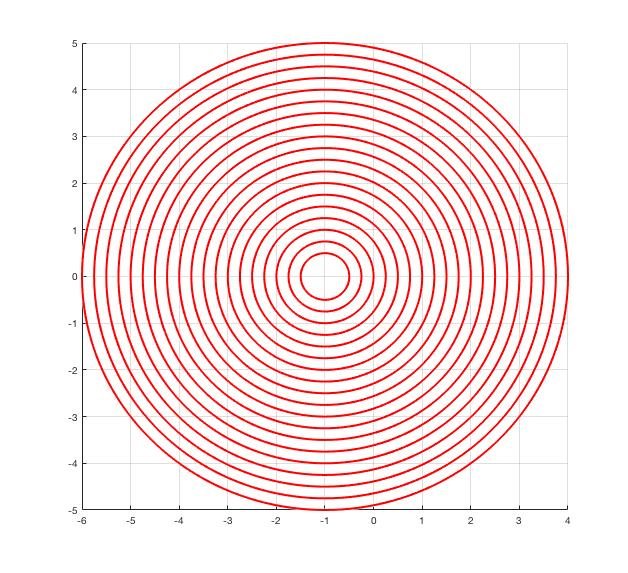
\includegraphics[scale=0.3]{lista2_1.jpeg}
				\caption{$\boldsymbol{\mu_{1}}$}
			\end{figure}
		\end{frame}
	
		\begin{frame}
			\frametitle{Questão 8}
			\begin{figure}[h]
				\centering
				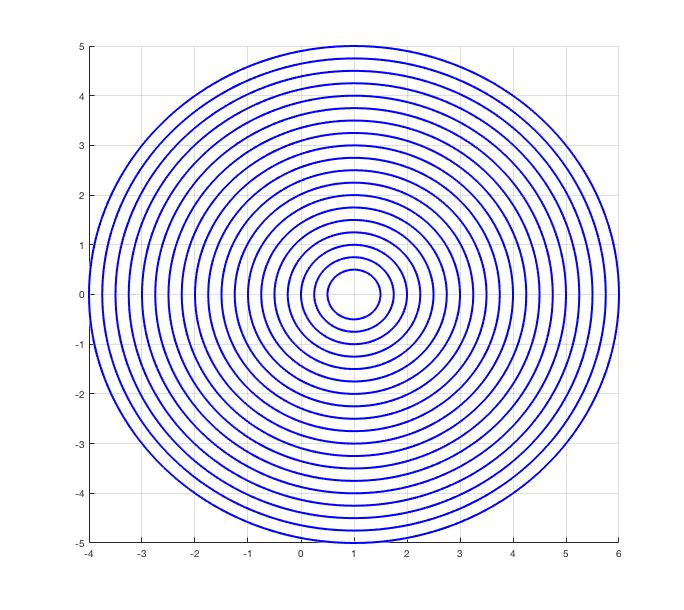
\includegraphics[scale=0.3]{lista2_2.jpeg}
				\caption{$\boldsymbol{\mu_{2}}$}
			\end{figure}
		\end{frame}
		
		\begin{frame}
			\frametitle{Questão 8}
			\begin{figure}[h]
				\centering
				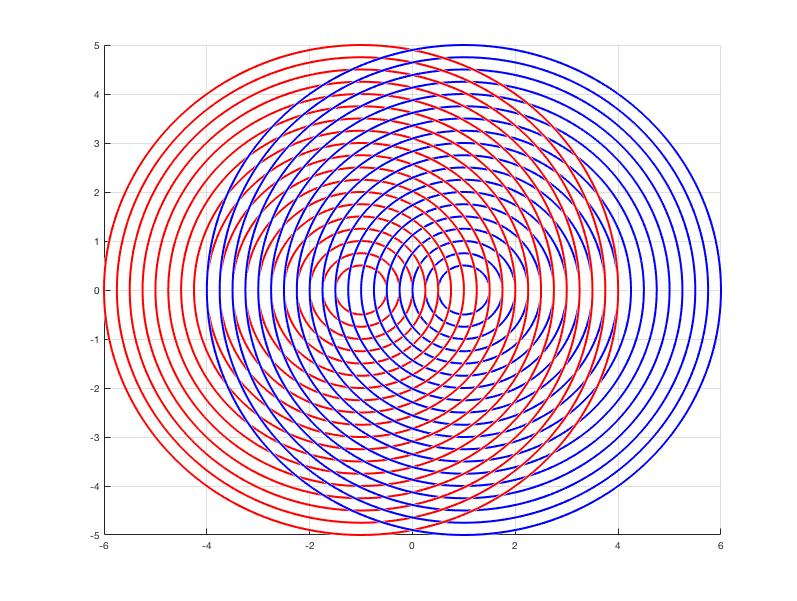
\includegraphics[scale=0.3]{lista2_3.jpeg}
				\caption{$\boldsymbol{\mu_{2}}$ e $\boldsymbol{\mu_{2}}$}
			\end{figure}
		\end{frame}
	
		\begin{frame}
			\frametitle{Questão 8}
			Calculando a função de \textbf{Máxima Verossimilhança(ML)} $\Lambda_{ML}(x)$:
			$$\Lambda_{ML}(x) = \frac{f(\boldsymbol{x}|C_{2})}{f(\boldsymbol{x}|C_{1})} \overset{C_{2}}{>} \underset{C_{1}}{<} \frac{f(C_{1})}{f(C_{2})}$$
			Tomando $C_{1}$ e $C_{2}$ como equiprováveis temos:
			$\Lambda_{ML}(x)$:
			$$\Lambda_{ML}(x) = \frac{f(\boldsymbol{x}|C_{2})}{f(\boldsymbol{x}|C_{1})} \overset{C_{2}}{>} \underset{C_{1}}{<} 1$$
		\end{frame}
		
		\begin{frame}
			\frametitle{Questão 8}
			Assim:
			\begin{align*}
				\Lambda_{ML}(x) &= \frac{\frac{1}{(2\pi)^{D/2}det(\boldsymbol{C})^{1/2}}exp(-\frac{1}{2}(\boldsymbol{x} - \boldsymbol{\mu_{2}})^{T}\boldsymbol{C}^{-1}(\boldsymbol{x} - \boldsymbol{\mu_{2}}))}{\frac{1}{(2\pi)^{D/2}det(\boldsymbol{C})^{1/2}}exp(-\frac{1}{2}(\boldsymbol{x} - \boldsymbol{\mu_{1}})^{T}\boldsymbol{C}^{-1}(\boldsymbol{x} - \boldsymbol{\mu_{1}}))}\overset{C_{2}}{>} \underset{C_{1}}{<} 1\\
				\\
				&= \frac{exp(-\frac{1}{2}(\boldsymbol{x} - \boldsymbol{\mu_{2}})^{T}\boldsymbol{C}^{-1}(\boldsymbol{x} - \boldsymbol{\mu_{2}}))}{exp(-\frac{1}{2}(\boldsymbol{x} - \boldsymbol{\mu_{1}})^{T}\boldsymbol{C}^{-1}(\boldsymbol{x} - \boldsymbol{\mu_{1}}))}\overset{C_{2}}{>} \underset{C_{1}}{<} 1\\
				\\
				&=exp(-\frac{1}{2}(\boldsymbol{x} - \boldsymbol{\mu_{2}})^{T}\boldsymbol{C}^{-1}(\boldsymbol{x} - \boldsymbol{\mu_{2}}) + \frac{1}{2}(\boldsymbol{x} - \boldsymbol{\mu_{1}})^{T}\boldsymbol{C}^{-1}(\boldsymbol{x} - \boldsymbol{\mu_{1}}))\\
				\Lambda_{ML}(x) &= exp-\frac{1}{2}\{(\boldsymbol{x} - \boldsymbol{\mu_{2}})^{T}\boldsymbol{C}^{-1}(\boldsymbol{x} - \boldsymbol{\mu_{2}}) - [(\boldsymbol{x} - \boldsymbol{\mu_{1}})^{T}\boldsymbol{C}^{-1}(\boldsymbol{x} - \boldsymbol{\mu_{1}})]\}
			\end{align*}
		\end{frame}
		
		\begin{frame}
			\frametitle{Questão 8}
			Calculando o \textbf{logaritmo de Verossimilhança} $\delta_{ML}(\Lambda_{ML}(x))$:
			\begin{align*}
				\ln[\Lambda_{ML}(x)] &= \ln{e^{-\frac{1}{2}\{(\boldsymbol{x} - \boldsymbol{\mu_{2}})^{T}\boldsymbol{C}^{-1}(\boldsymbol{x} - \boldsymbol{\mu_{2}}) - [(\boldsymbol{x} - \boldsymbol{\mu_{1}})^{T}\boldsymbol{C}^{-1}(\boldsymbol{x} - \boldsymbol{\mu_{1}})]\}}}\\
				&= -\frac{1}{2}\{(\boldsymbol{x} - \boldsymbol{\mu_{2}})^{T}\boldsymbol{C}^{-1}(\boldsymbol{x} - \boldsymbol{\mu_{2}}) - [(\boldsymbol{x} - \boldsymbol{\mu_{1}})^{T}\boldsymbol{C}^{-1}(\boldsymbol{x} - \boldsymbol{\mu_{1}})]\}\\
			\end{align*}
			Expandindo os produtos:
			\begin{align*}
				\delta_{ML}(\Lambda_{ML}(x)= &-\frac{1}{2}\{ \boldsymbol{x}^{T}\boldsymbol{C}^{-1}\boldsymbol{x} - \boldsymbol{x}^{T}\boldsymbol{C}^{-1}\boldsymbol{\mu_{2}} - \boldsymbol{\mu_{2}}^{T}\boldsymbol{C}^{-1}\boldsymbol{x} - 
				\boldsymbol{\mu_{2}}^{T}\boldsymbol{C}^{-1}\boldsymbol{\mu_{2}}\\
				&-[\boldsymbol{x}^{T}\boldsymbol{C}^{-1}\boldsymbol{x} - 
				\boldsymbol{x}^{T}\boldsymbol{C}^{-1}\boldsymbol{\mu_{1}} - 
				\boldsymbol{\mu_{1}}^{T}\boldsymbol{C}^{-1}\boldsymbol{x} + 
				\boldsymbol{\mu_{1}}^{T}\boldsymbol{C}^{-1}\boldsymbol{\mu_{1}}]\}
			\end{align*}
		\end{frame}
	
		\begin{frame}
			\frametitle{Questão 8}
			\begin{align*}
				\delta_{ML}(\Lambda_{ML}(x)= &-\frac{1}{2}\{ \cancel{\boldsymbol{x}^{T}\boldsymbol{C}^{-1}\boldsymbol{x}} - \boldsymbol{x}^{T}\boldsymbol{C}^{-1}\boldsymbol{\mu_{2}} - \boldsymbol{\mu_{2}}^{T}\boldsymbol{C}^{-1}\boldsymbol{x} + 
				\boldsymbol{\mu_{2}}^{T}\boldsymbol{C}^{-1}\boldsymbol{\mu_{2}}\\
				&\cancel{-\boldsymbol{x}^{T}\boldsymbol{C}^{-1}\boldsymbol{x}} + 
				\boldsymbol{x}^{T}\boldsymbol{C}^{-1}\boldsymbol{\mu_{1}} + 
				\boldsymbol{\mu_{1}}^{T}\boldsymbol{C}^{-1}\boldsymbol{x} - 
				\boldsymbol{\mu_{1}}^{T}\boldsymbol{C}^{-1}\boldsymbol{\mu_{1}}\}\\
				=&-\frac{1}{\cancel{2}}\{ -\cancel{2}\boldsymbol{\mu_{2}}^{T}\boldsymbol{C}^{-1}\boldsymbol{x}
				+ \cancel{2}\boldsymbol{\mu_{1}}^{T}\boldsymbol{C}^{-1}\boldsymbol{x}\ - 
			    [\boldsymbol{\mu_{1}}^{T}\boldsymbol{C}^{-1}\boldsymbol{\mu_{1}}\\ &- 
			    \boldsymbol{\mu_{2}}^{T}\boldsymbol{C}^{-1}\boldsymbol{\mu_{2}}]\}\\
			    =&\boldsymbol{\mu_{2}}^{T}\boldsymbol{C}^{-1}\boldsymbol{x} - \boldsymbol{\mu_{1}}^{T}\boldsymbol{C}^{-1}\boldsymbol{x} + \frac{1}{2}[\boldsymbol{\mu_{1}}^{T}\boldsymbol{C}^{-1}\boldsymbol{\mu_{1}}\\ &- 
			    \boldsymbol{\mu_{2}}^{T}\boldsymbol{C}^{-1}\boldsymbol{\mu_{2}}]\\
			    =&(\boldsymbol{\mu_{2}}^{T}\boldsymbol{C}^{-1} - \boldsymbol{\mu_{1}}^{T}\boldsymbol{C}^{-1})\boldsymbol{x}+\frac{1}{2}[\boldsymbol{\mu_{1}}^{T}\boldsymbol{C}^{-1}\boldsymbol{\mu_{1}} - \boldsymbol{\mu_{2}}^{T}\boldsymbol{C}^{-1}\boldsymbol{\mu_{2}}]
			\end{align*}
		\end{frame}
	
		\begin{frame}
			\frametitle{Questão 8}
			Fazendo: $$\boldsymbol{w^{T}} = (\boldsymbol{\mu_{2}}^{T}\boldsymbol{C}^{-1} - \boldsymbol{\mu_{1}}^{T}\boldsymbol{C}^{-1})$$ e: $$\boldsymbol{w_{0}} = \frac{1}{2}[\boldsymbol{\mu_{1}}^{T}\boldsymbol{C}^{-1}\boldsymbol{\mu_{1}} - \boldsymbol{\mu_{2}}^{T}\boldsymbol{C}^{-1}\boldsymbol{\mu_{2}}]$$ temos:
			$$\ln[\Lambda_{ML}(x)] = \boldsymbol{w^{T}}\boldsymbol{x} + \boldsymbol{w_{0}}$$
			o que, pela linearidade em $\boldsymbol{x}$ da nova equação, configura a equação de um \textbf{hiperplano}.
		\end{frame}
\end{document}








